
\section{From algorithm to physical realization}
\subsection{Programming stack}
%%%%%%%%%%%%%%%%%%%%%%%%%%%%%%%%%%%%%%%%%%%%%%%%%%%%%%%%%%%%%%%%%%%%%%%%%%%%%%%%
\begin{frame}{Programming stack}
	\centering
	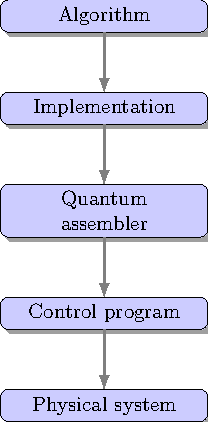
\includegraphics[scale=0.85]{pics/stack.pdf}
\end{frame}
%%%%%%%%%%%%%%%%%%%%%%%%%%%%%%%%%%%%%%%%%%%%%%%%%%%%%%%%%%%%%%%%%%%%%%%%%%%%%%%%
\subsection{QuTiP implementation}
\begin{frame}[fragile]{Implementation}
	QuTiP implementation of Deutsch's algorithm for function $f(0) = 1, f(1) = 0$.

	\begin{lstlisting}[language=Python]
qc = QubitCircuit(2, num_cbits=1)
qc.add_gate("X", 1)
qc.add_gate("SNOT", 1)
qc.add_gate("SNOT", 0)
qc.add_gate("CNOT", 1, 0)
qc.add_gate("X", 1)
qc.add_gate("SNOT", 0)
qc.add_measurement("M0", targets=[0], classical_store=0)
	\end{lstlisting}
\end{frame}
%%%%%%%%%%%%%%%%%%%%%%%%%%%%%%%%%%%%%%%%%%%%%%%%%%%%%%%%%%%%%%%%%%%%%%%%%%%%%%%%
\subsection{Quantum assembler}
\begin{frame}[fragile]{Quantum assembler}
	\lstinputlisting{deutsch4.qasm}
\end{frame}
%%%%%%%%%%%%%%%%%%%%%%%%%%%%%%%%%%%%%%%%%%%%%%%%%%%%%%%%%%%%%%%%%%%%%%%%%%%%%%%%
\subsection{Quantum physical system}
\begin{frame}{Physical system}
\begin{block}{Schr\"odinger equation}
	\centering
	\huge
	$i \hbar \frac{\partial \Psi(t)}{\partial t} = \hat H \Psi(t)$
\end{block}
\vspace{1cm}
\begin{itemize}
\item  $H$ is a Hermitian operator (\textit{i.e.} $H=H^\dagger$) called
	\textbf{Hamiltonian} of the system. 
\item  $\Psi(t)$ is a \textit{wave function} of the system
\item $\hbar$ is the reduced Planck constant
\end{itemize}	
\end{frame}


\begin{frame}{Physical system}W
\begin{block}{Solution to the Schrödinger equation:}
\begin{large}
$$
\ket{\psi_{t_1}} = U(t_0, t_1) \ket{\psi_{t_0}},
$$
\end{large}
where
\begin{itemize}
\item $\ket{\psi_{t_0}}$ --- initial state of the system, 
\item $\ket{\psi_{t_1}}$ --- final state of the system
\item $U(t_0, t_1)$ --- \textbf{unitary operator} driving the system from 
$t_0$ to $t_1$. 
\end{itemize}
\end{block}

\begin{itemize}
\item An operator is unitary iff $UU^\dagger=U^\dagger U=\mathbb{1}$
\framebreak
\item If Hamiltonian $H$ is constant between time $t_0$ and $t_1$, then:
$$
U(t_0, t_1) = e^{-i (t_1-t_0) H },
$$
where $e^M=\sum_{k=0}^\infty \frac{M^k}{k!}$.
\end{itemize}
\end{frame}
%%%%%%%%%%%%%%%%%%%%%%%%%%%%%%%%%%%%%%%%%%%%%%%%%%%%%%%%%%%%%%%%%%%%%%%%%%%%%%%%
\begin{frame}{Physical system}
	\begin{center}
		$H(t) = h_{x_0}(t)\sigma_x^0+
			h_{x_1}(t)\sigma_x^1+
			h_{z_0}(t)\sigma_z^0+
			h_{z_1}(t)\sigma_z^1+
			J(t)\left(\sigma_x^0\sigma_x^{1} + \sigma_y^0\sigma_y^{1}\right)$\\[1cm]
		\includegraphics[width=0.35\textwidth, page=2]{pics/bloch_dynamics.pdf}
		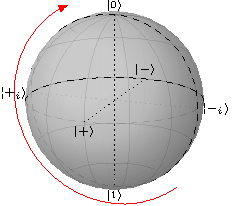
\includegraphics[width=0.35\textwidth, page=1]{pics/bloch_dynamics.pdf}
	\end{center}
\end{frame}
%%%%%%%%%%%%%%%%%%%%%%%%%%%%%%%%%%%%%%%%%%%%%%%%%%%%%%%%%%%%%%%%%%%%%%%%%%%%%%%%
\subsection{Steering the program}
\begin{frame}{Control program}
	\begin{center}
		$H(t) = h_{x_0}(t)\sigma_x^0+
			h_{x_1}(t)\sigma_x^1+
			h_{z_0}(t)\sigma_z^0+
			h_{z_1}(t)\sigma_z^1+
			J(t)\left(\sigma_x^0\sigma_x^{1} + \sigma_y^0\sigma_y^{1}\right)$\\[0.5cm]
		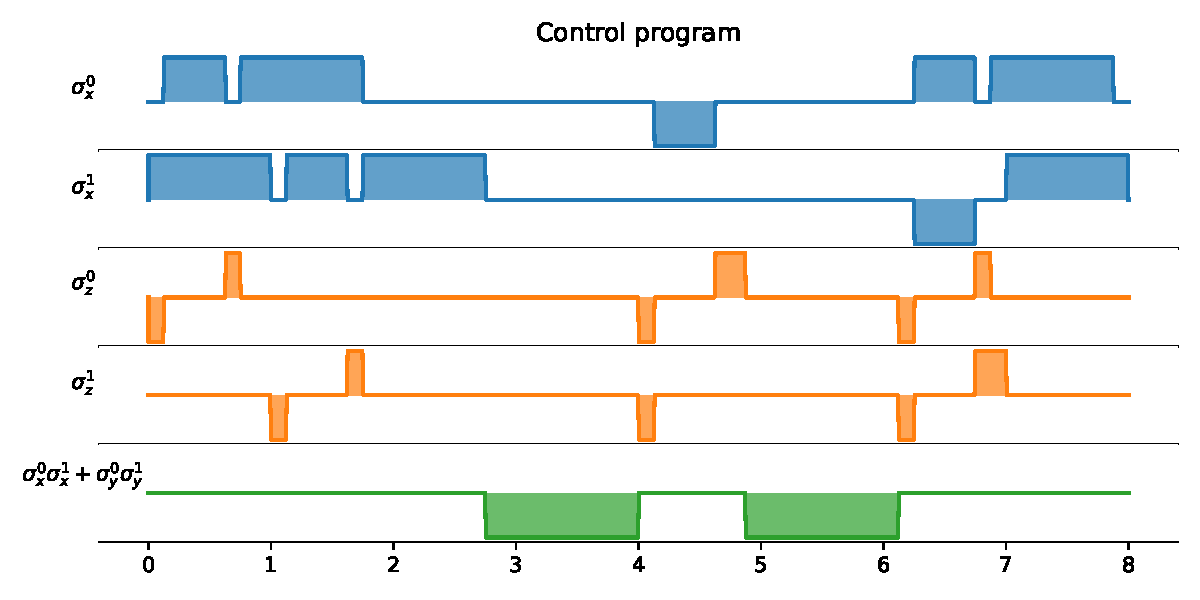
\includegraphics[height=0.55\textheight]{../src/control.pdf}
	\end{center}
\end{frame}
%%%%%%%%%%%%%%%%%%%%%%%%%%%%%%%%%%%%%%%%%%%%%%%%%%%%%%%%%%%%%%%%%%%%%%%%%%%%%%%%
\section{Problem of noisy devices}
\subsection{A zoo of quantum noisy channels}
%%%%%%%%%%%%%%%%%%%%%%%%%%%%%%%%%%%%%%%%%%%%%%%%%%%%%%%%%%%%%%%%%%%%%%%%%%%%%%%%
\begin{frame}{Qubit channels --- zoo}
	\only<1>{
	\begin{figure}
	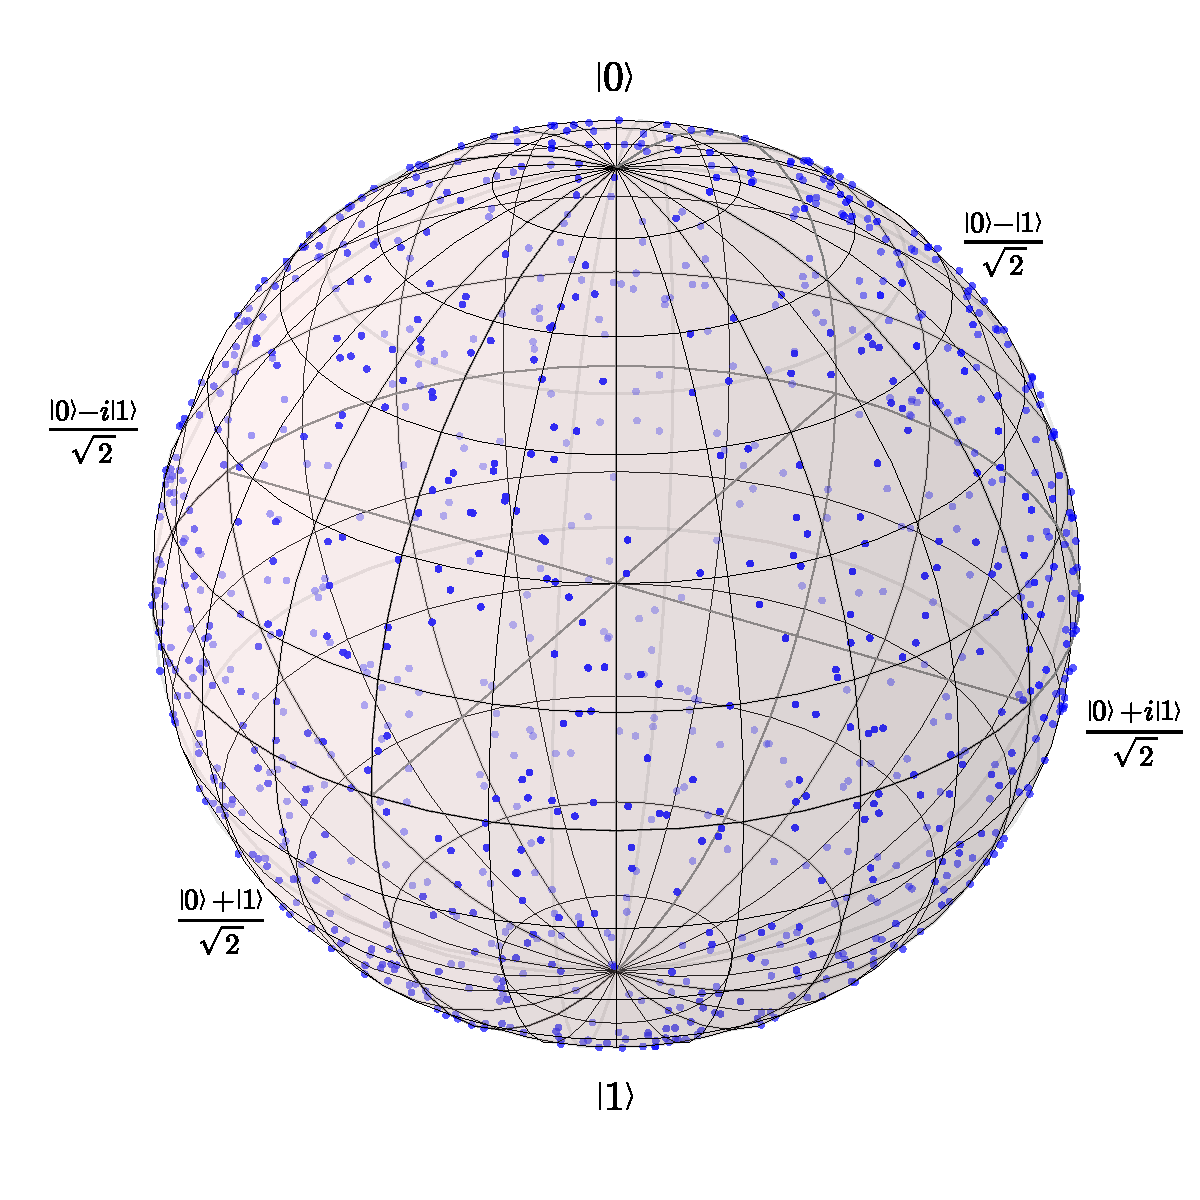
\includegraphics[height=0.75\textheight]{pics/channels/pure_states}
	\caption{Uniformly chosen 1000 random \alert{pure states}.}
	\end{figure}
	}
	% bit flip
	\only<2>{
	\begin{figure}
	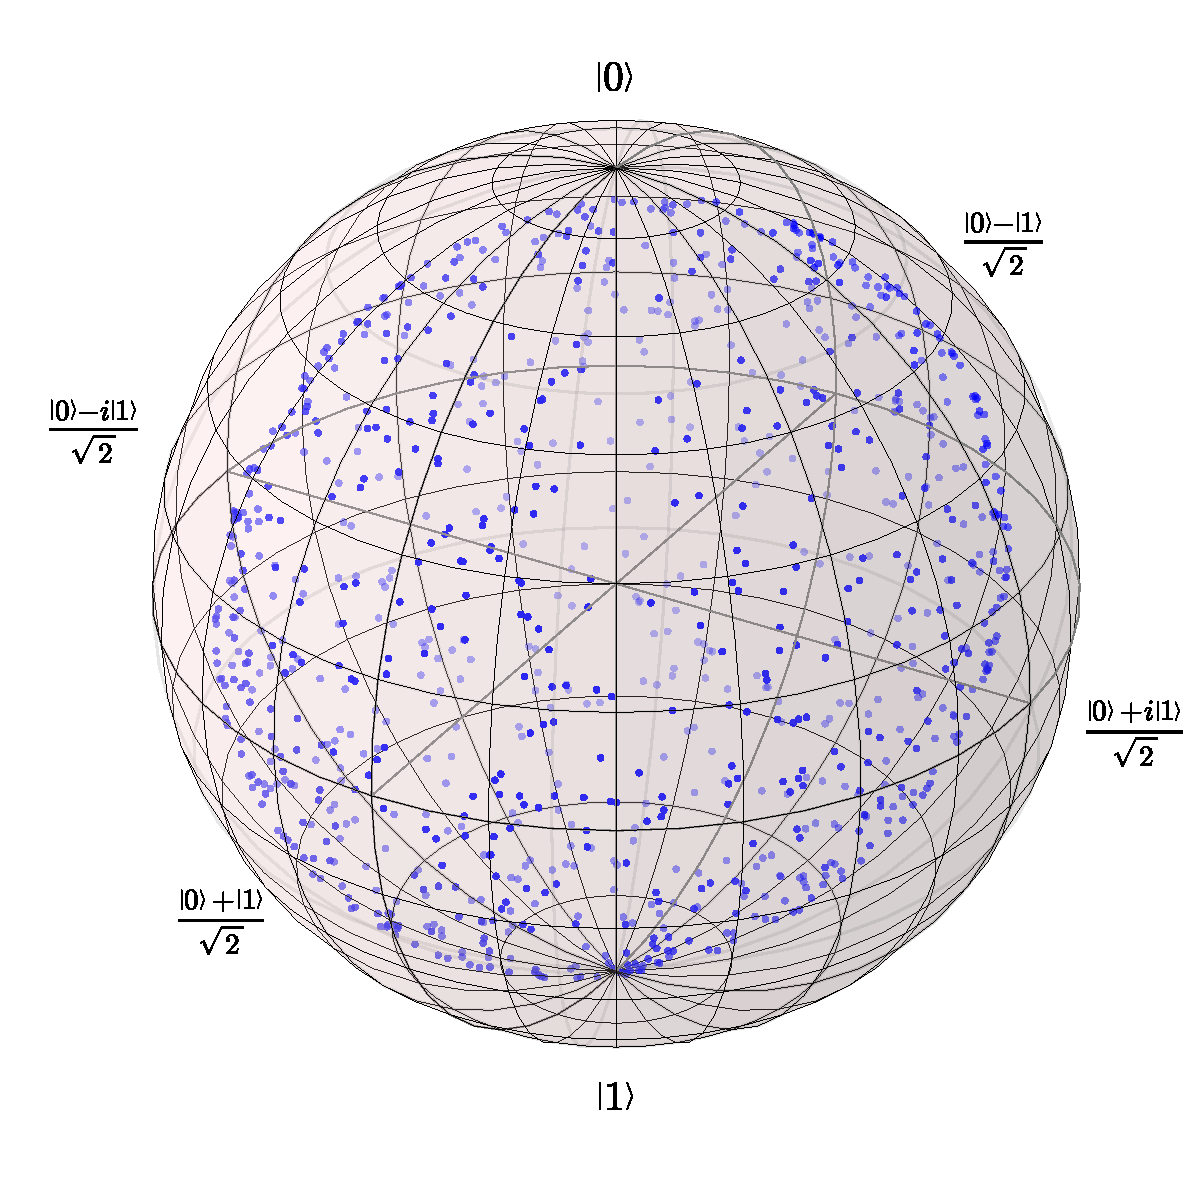
\includegraphics[height=0.75\textheight]{pics/channels/bitflip_0_1}
	\caption{Action of \alert{bit flip channel}: $\alert{p=0.1}$.}
	\end{figure}
	}
	%
	\only<3>{
	\begin{figure}
	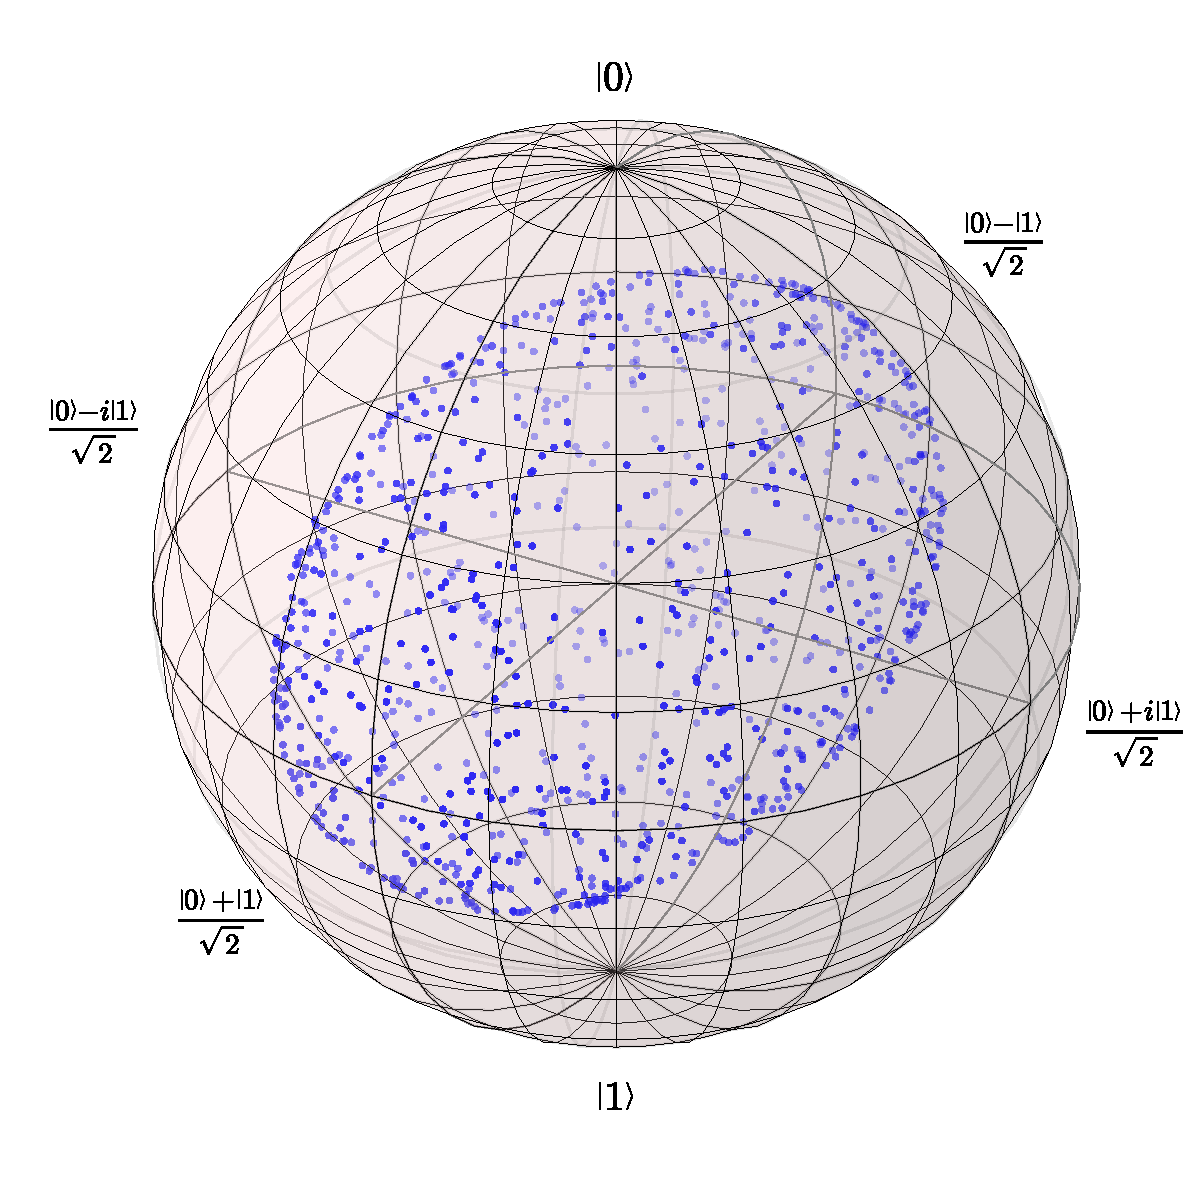
\includegraphics[height=0.75\textheight]{pics/channels/bitflip_0_2}
	\caption{Action of bit flip channel: $\alert{p=0.2}$.}
	\end{figure}
	}
	%
	\only<4>{
	\begin{figure}
	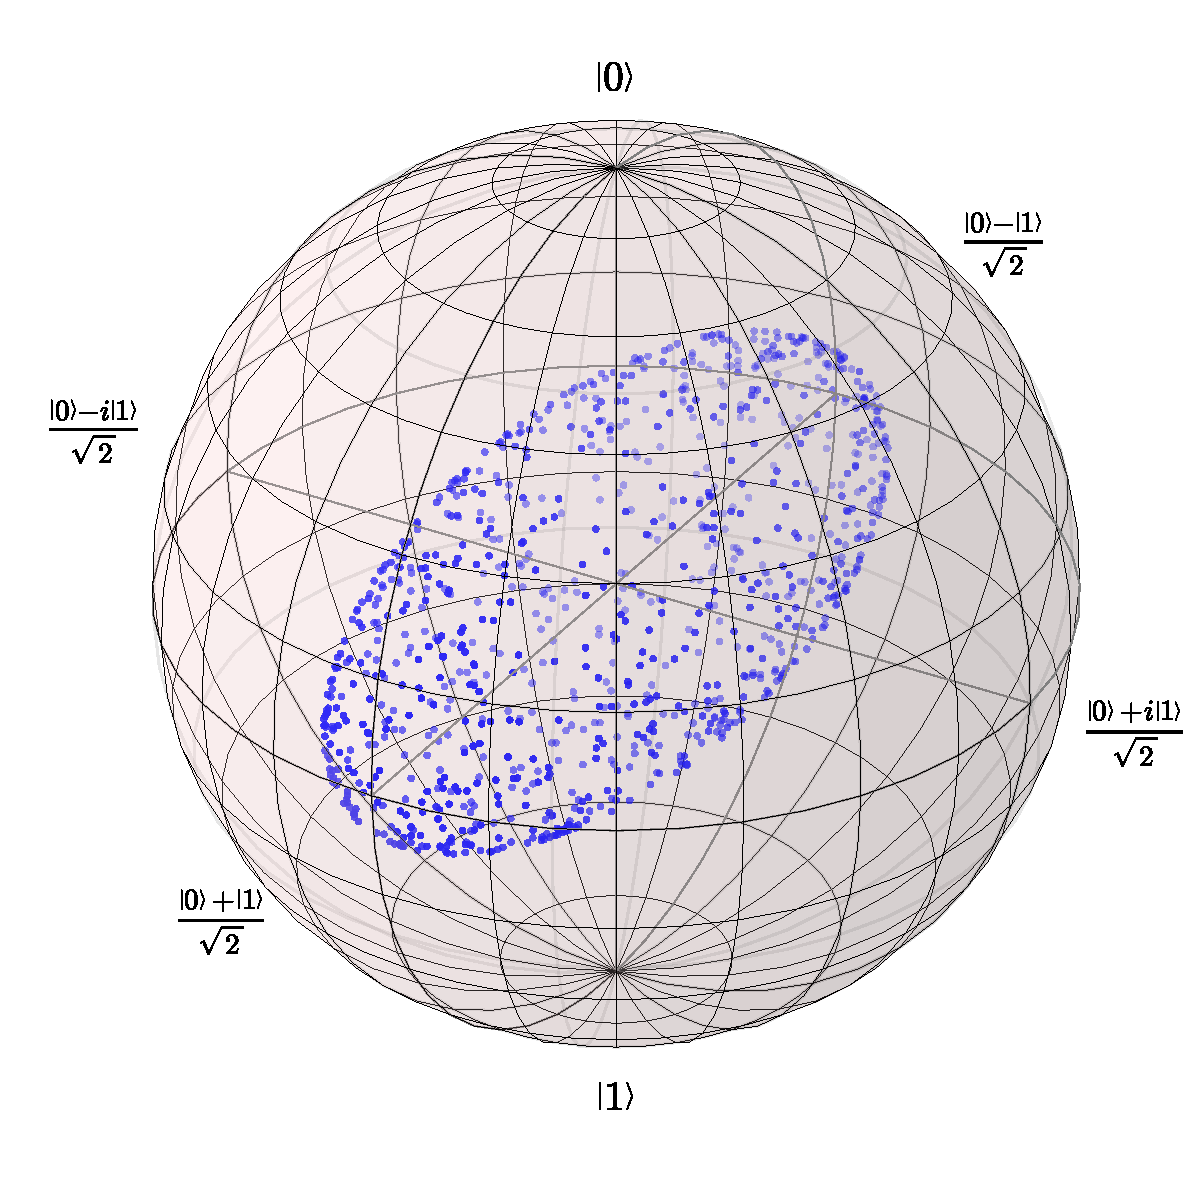
\includegraphics[height=0.75\textheight]{pics/channels/bitflip_0_3}
	\caption{Action of bit flip channel: $\alert{p=0.3}$.}
	\end{figure}
	}
	%
	\only<5>{
	\begin{figure}
	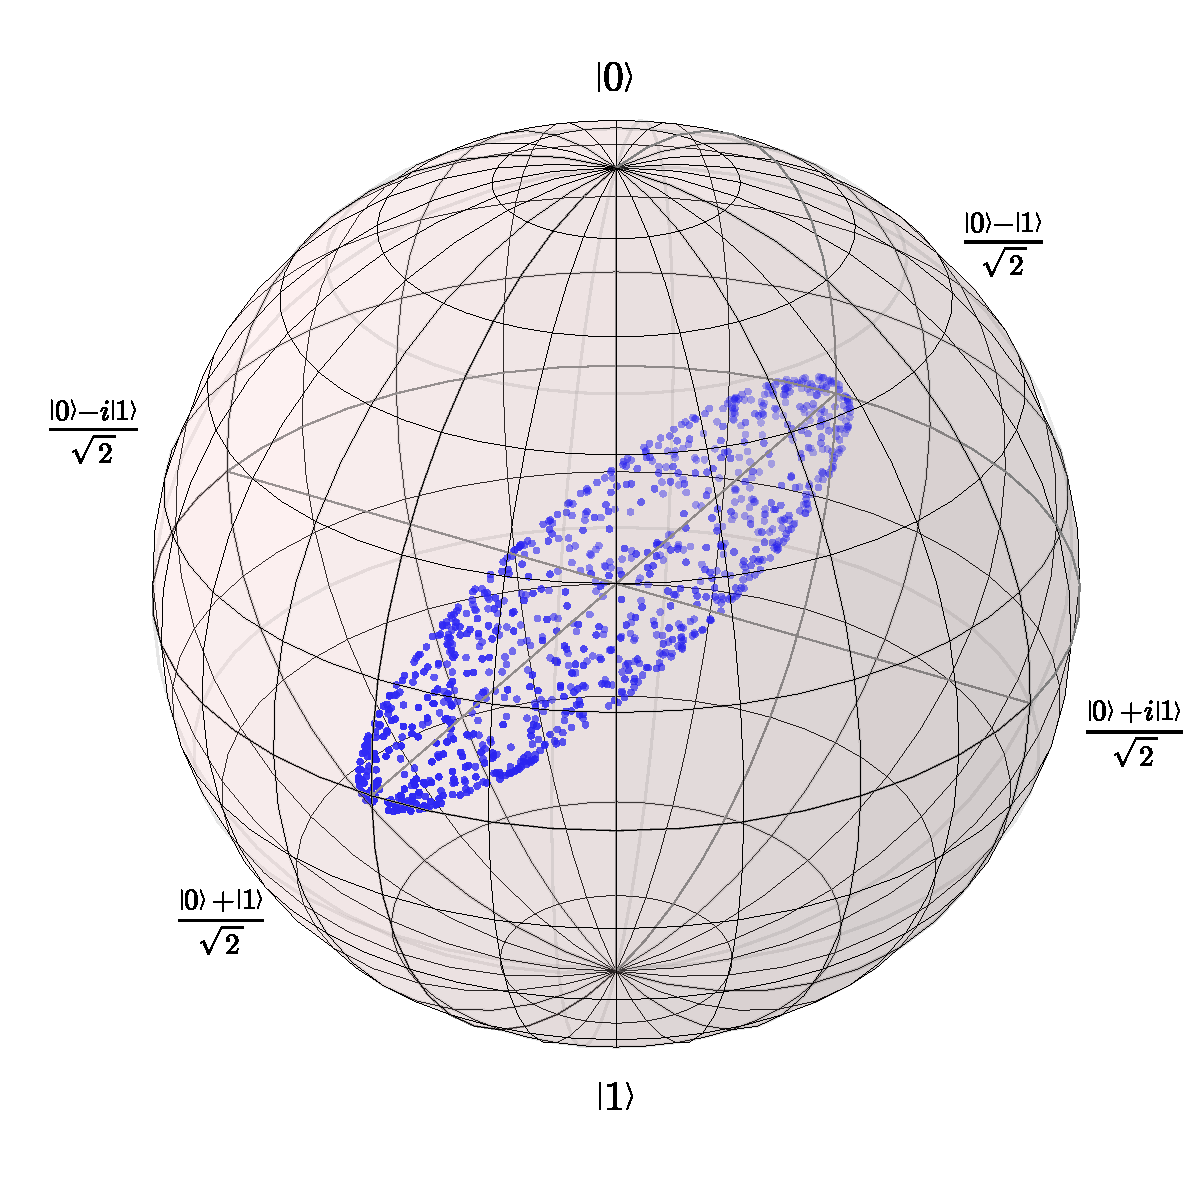
\includegraphics[height=0.75\textheight]{pics/channels/bitflip_0_4}
	\caption{Action of bit flip channel: $\alert{p=0.4}$.}
	\end{figure}
	}
	%
	\only<6>{
	\begin{figure}
	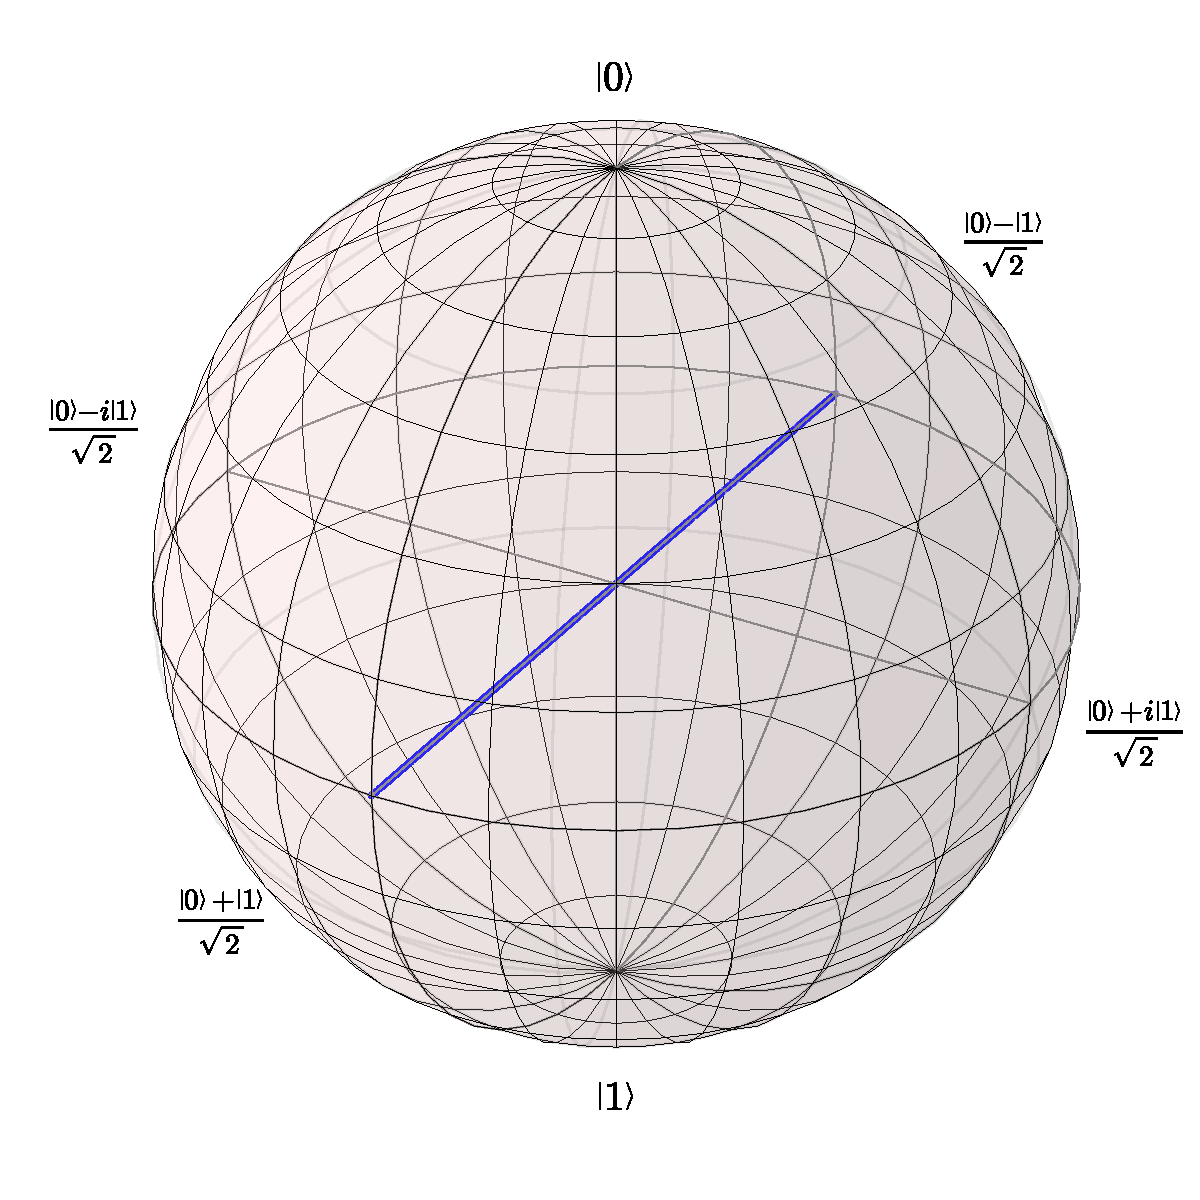
\includegraphics[height=0.75\textheight]{pics/channels/bitflip_0_5}
	\caption{Action of bit flip channel: $\alert{p=0.5}$.}
	\end{figure}
	}
	% phase flip
	\only<7>{
	\begin{figure}
	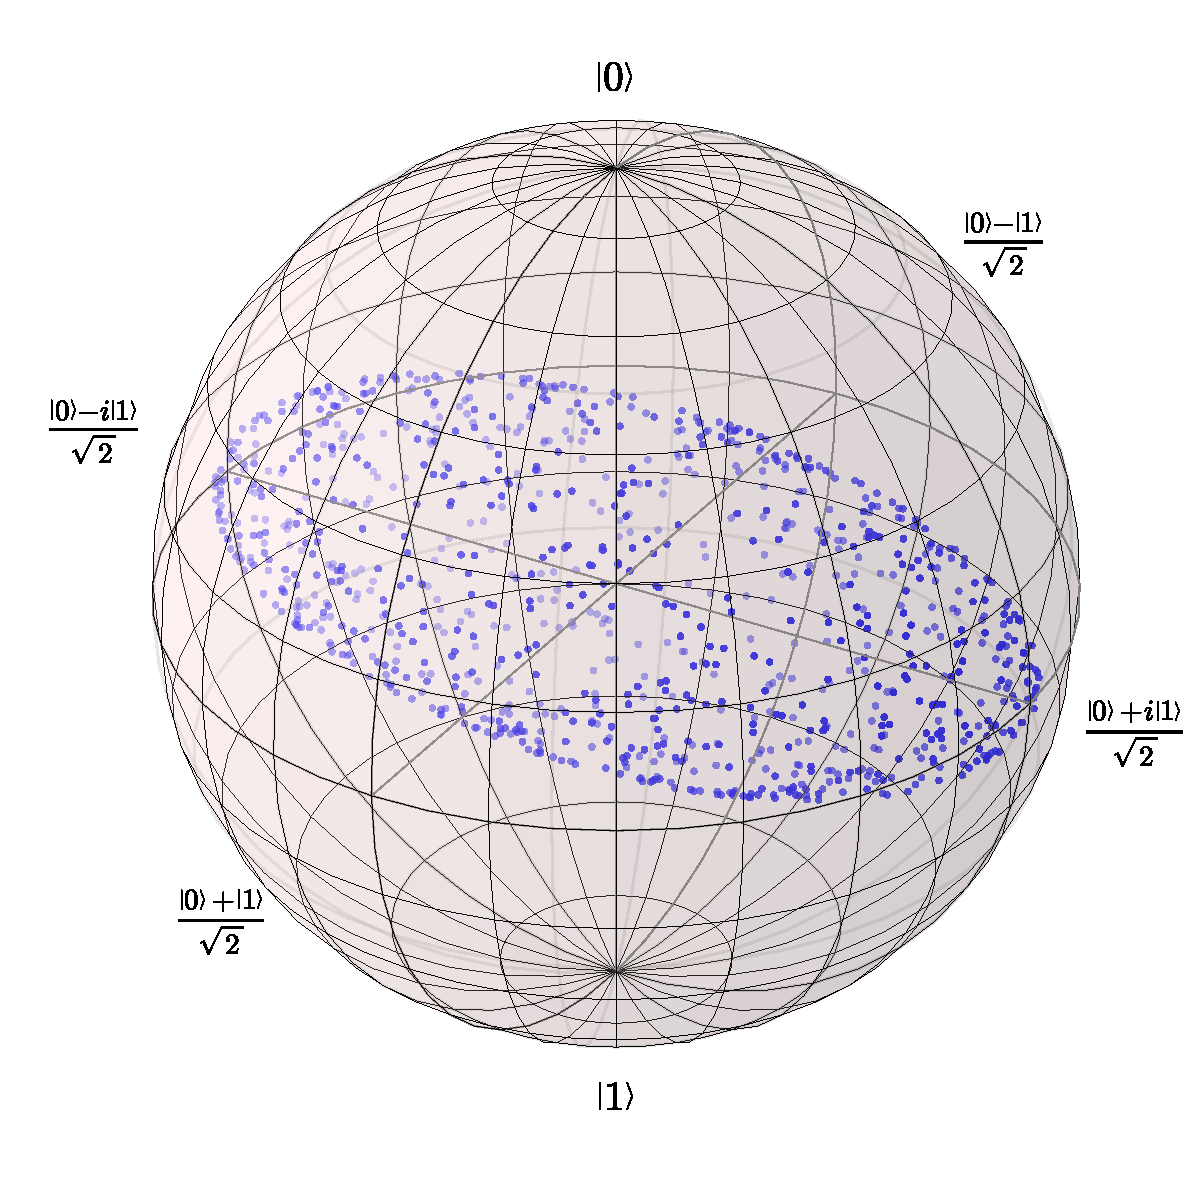
\includegraphics[height=0.75\textheight]{pics/channels/phaseflip_0_3}
	\caption{Action of \alert{phase flip channel}: $ p=0.3$.}
	\end{figure}
	}
	% bit phase flip
	\only<8>{
	\begin{figure}
	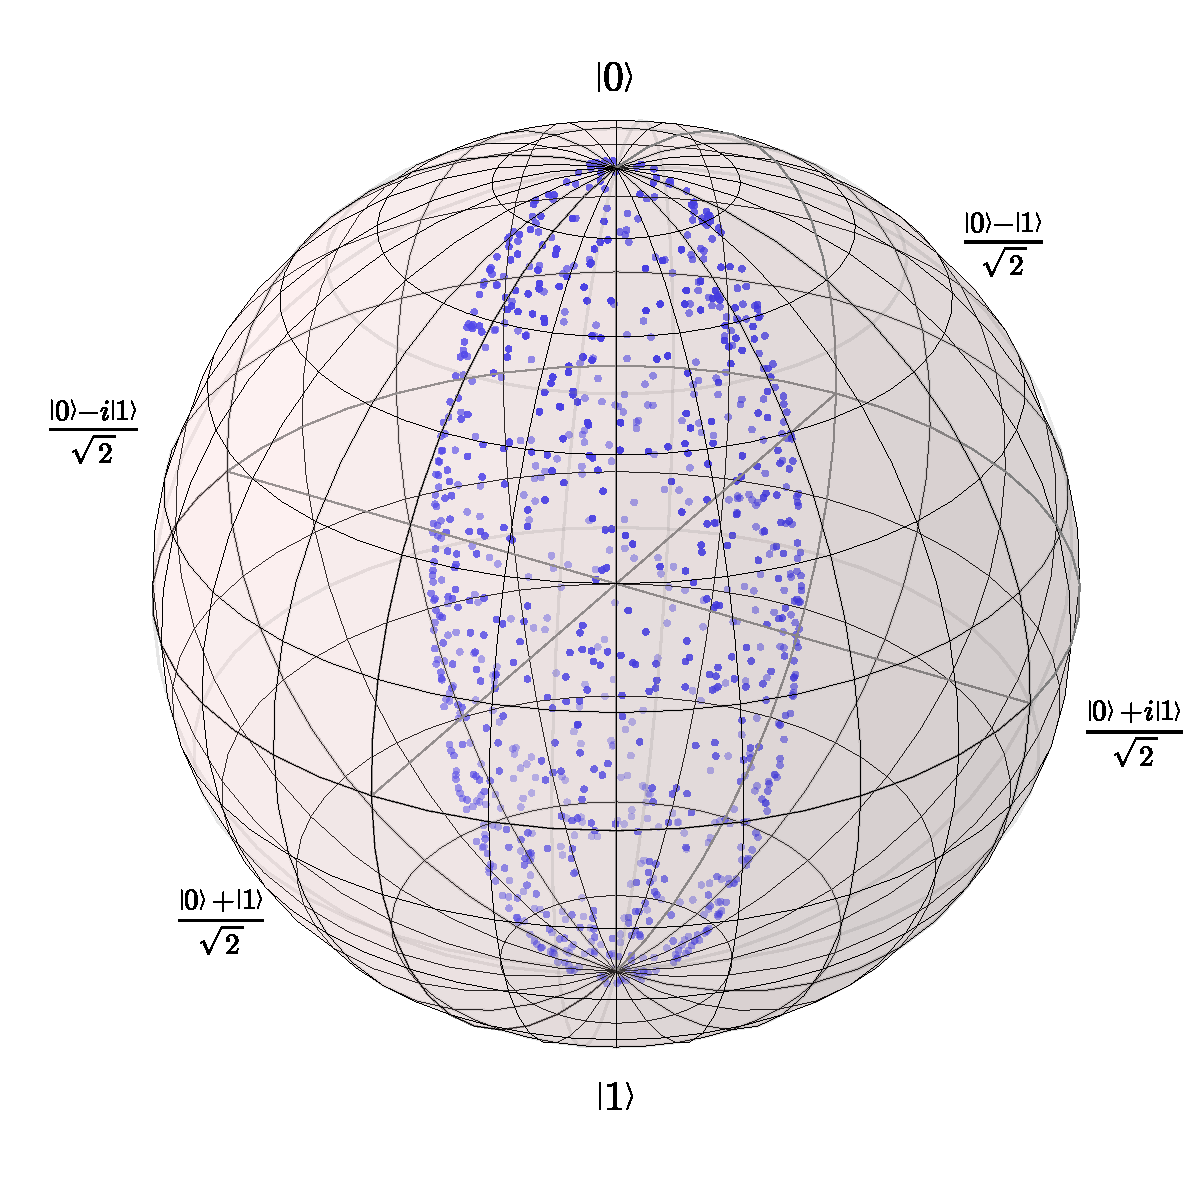
\includegraphics[height=0.75\textheight]{pics/channels/bitphaseflip_0_3}
	\caption{Action of \alert{bit-phase flip channel}: $p=0.3$.}
	\end{figure}
	}
	% amplitude dumping
	\only<9>{
	\begin{figure}
	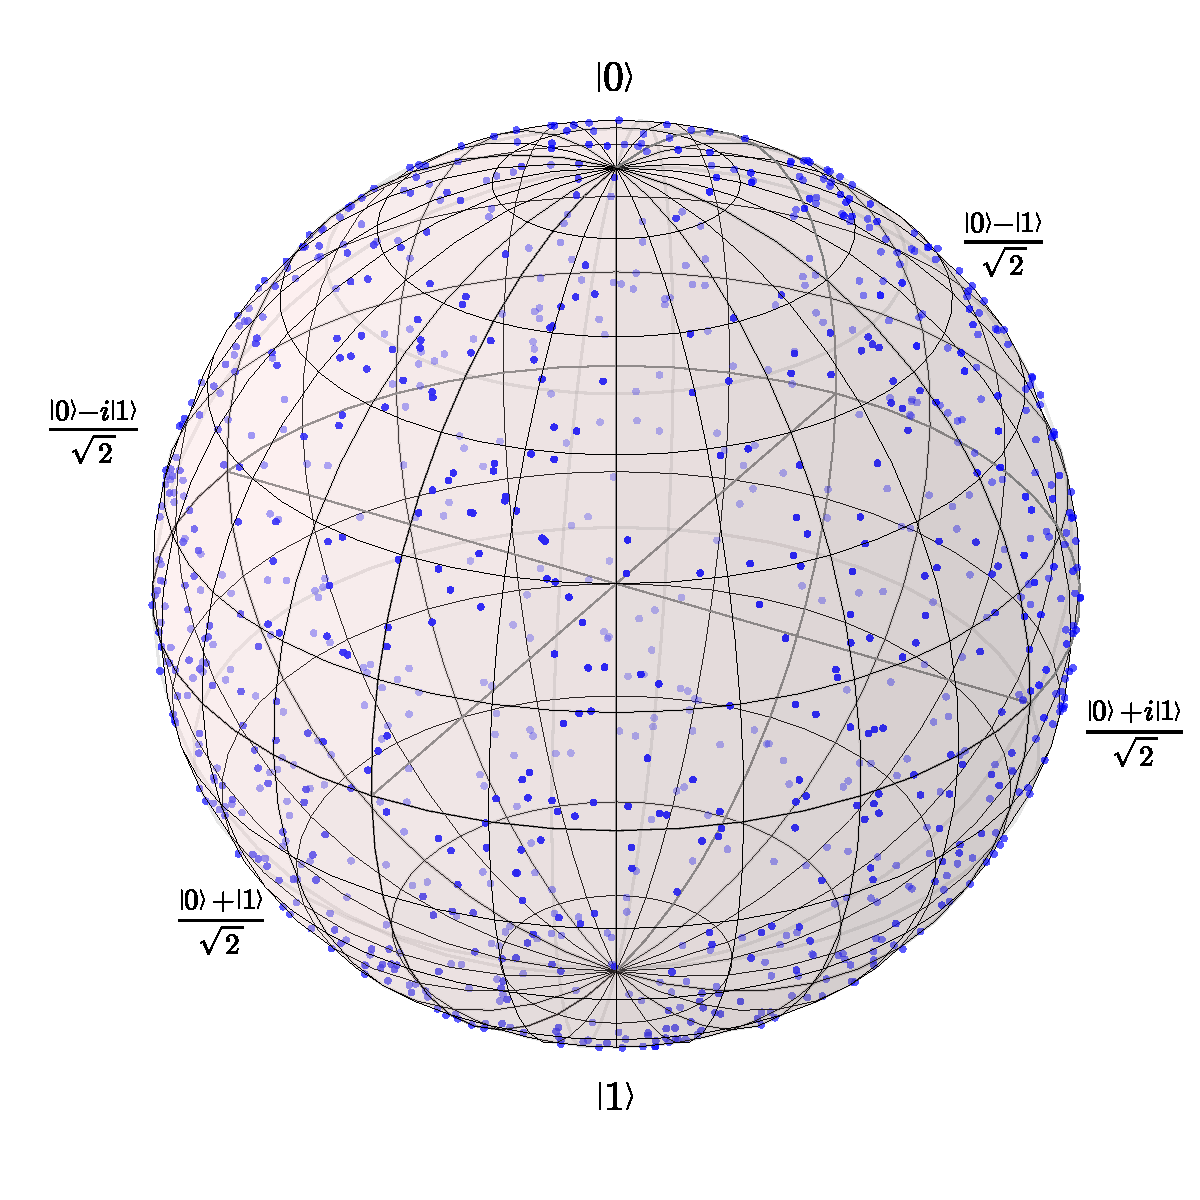
\includegraphics[height=0.75\textheight]{pics/channels/pure_states}
	\caption{Uniformly chosen 1000 random \alert{pure states}.}
	\end{figure}
	}
	\only<10>{
	\begin{figure}
	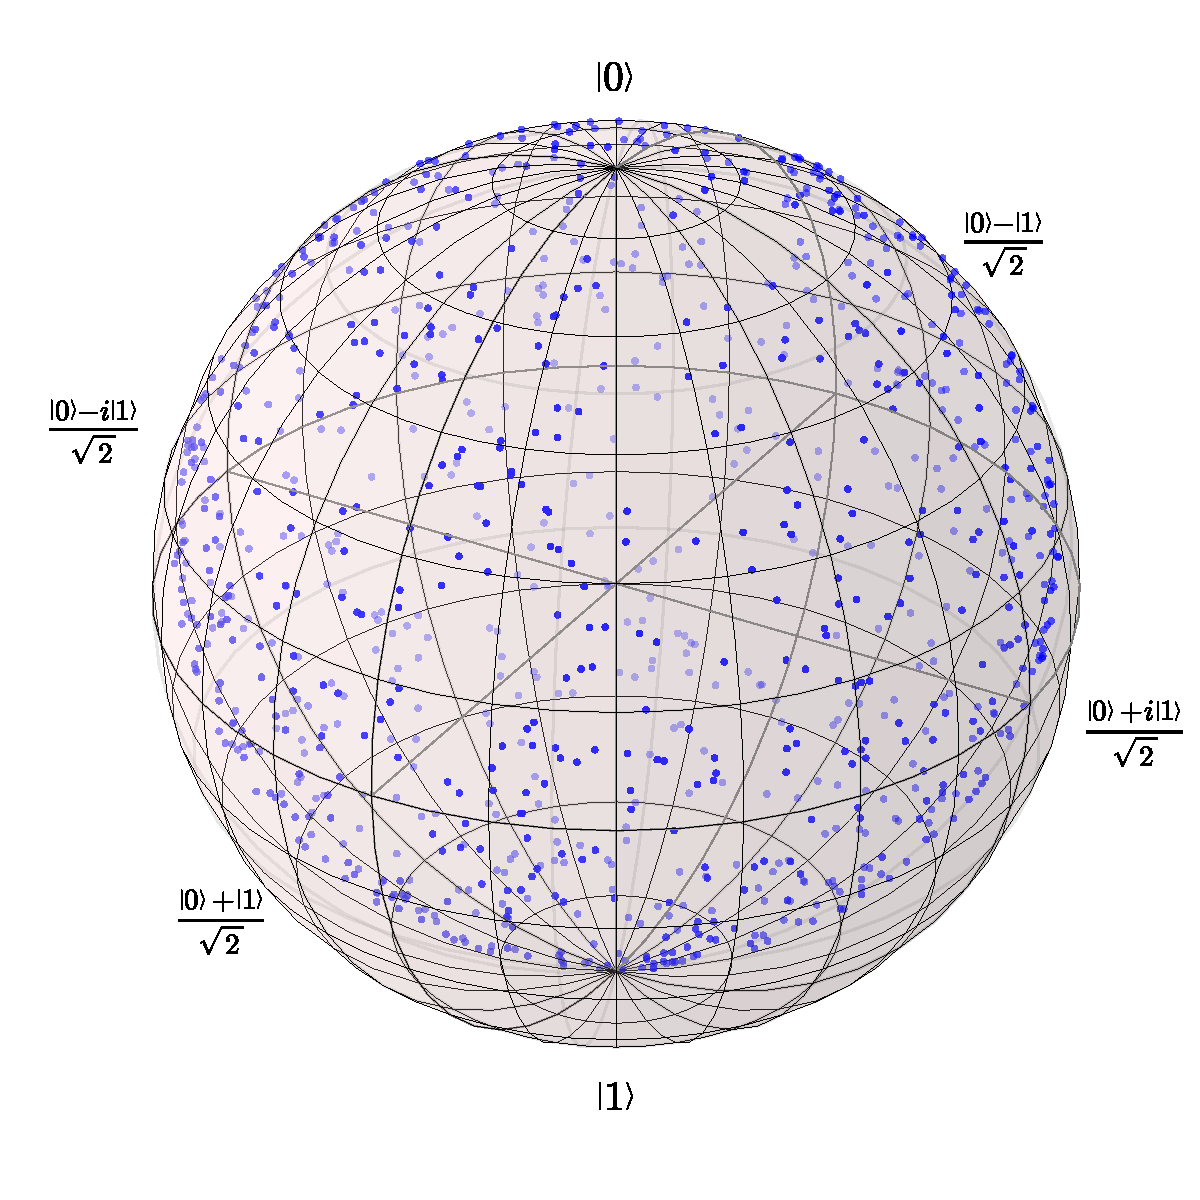
\includegraphics[height=0.75\textheight]{pics/channels/amplitude_dumping_0_1}
	\caption{
	Action of amplitude \alert{dumping channel}:  
	\alert{$p=0.1$}.
	}
	\end{figure}
	}
	%
	\only<11>{
	\begin{figure}
	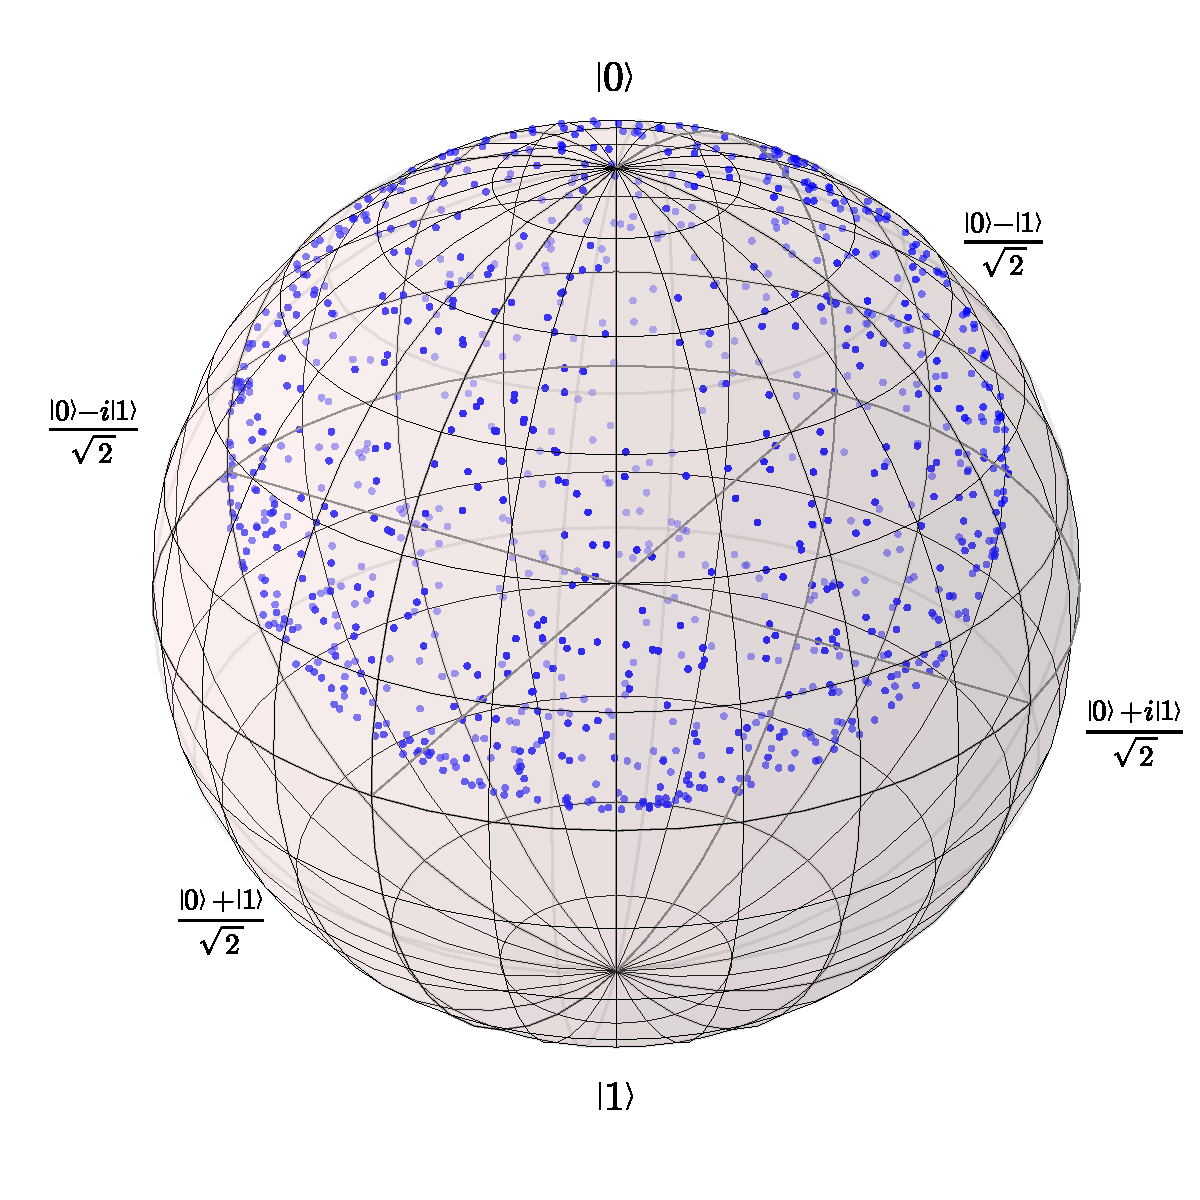
\includegraphics[height=0.75\textheight]{pics/channels/amplitude_dumping_0_3}
	\caption{
	Action of amplitude dumping channel:  
	\alert{$p=0.3$}.
	}
	\end{figure}
	}
	%
	\only<12>{
	\begin{figure}
	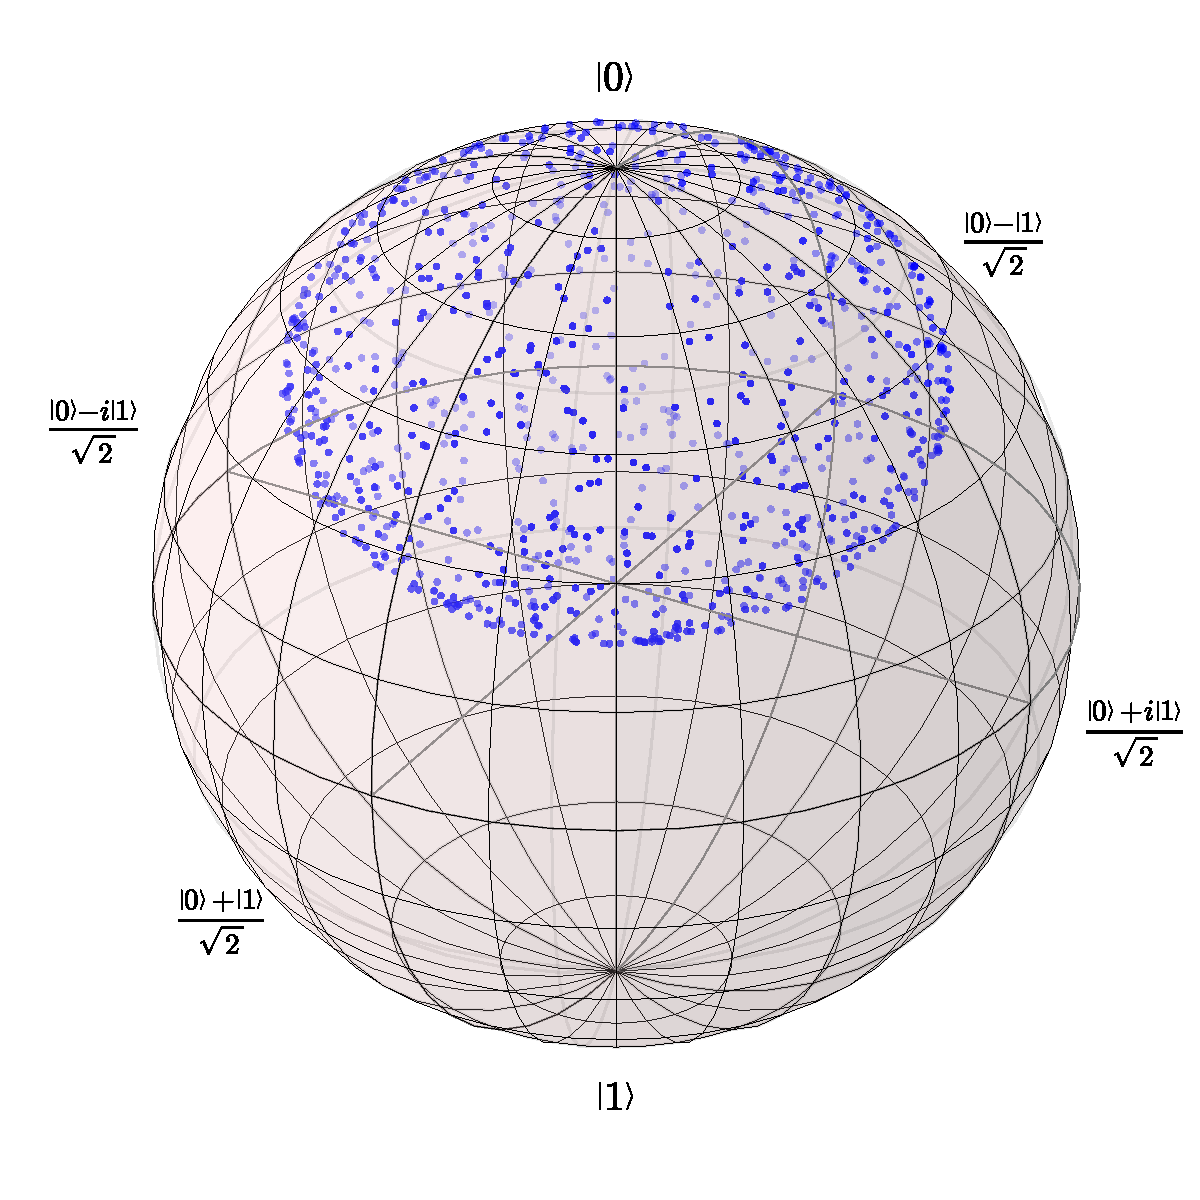
\includegraphics[height=0.75\textheight]{pics/channels/amplitude_dumping_0_5}
	\caption{
	Action of amplitude dumping channel:  
	\alert{$p=0.5$}.
	}
	\end{figure}
	}
	%
	\only<13>{
	\begin{figure}
	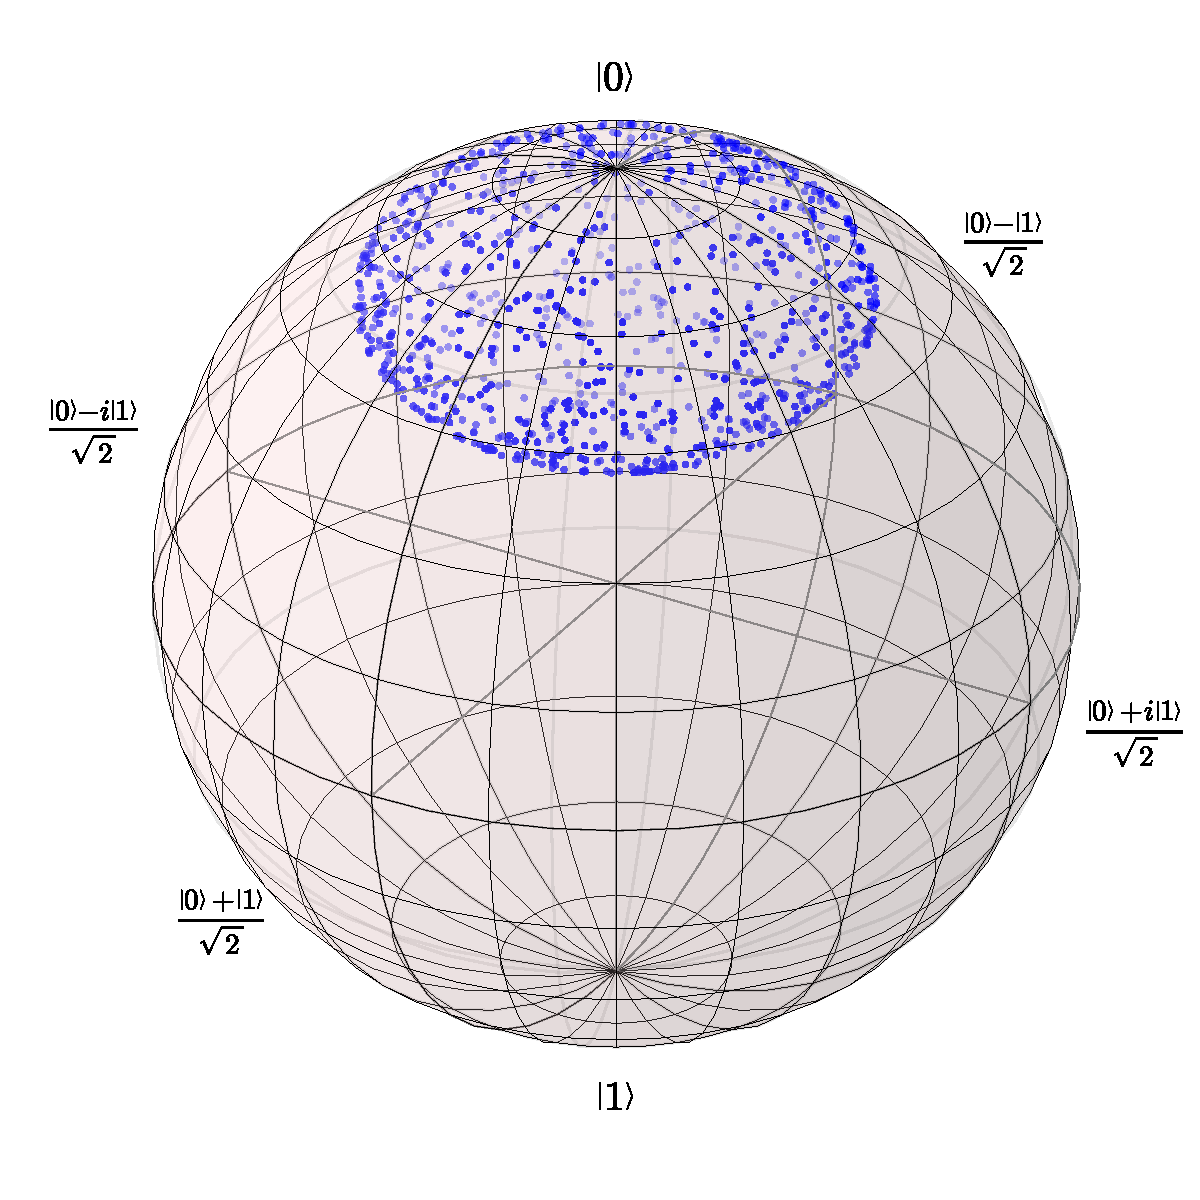
\includegraphics[height=0.75\textheight]{pics/channels/amplitude_dumping_0_7}
	\caption{
	Action of amplitude dumping channel:  
	\alert{$p=0.7$}.
	}
	\end{figure}
	}
	%
	\only<14>{
	\begin{figure}
	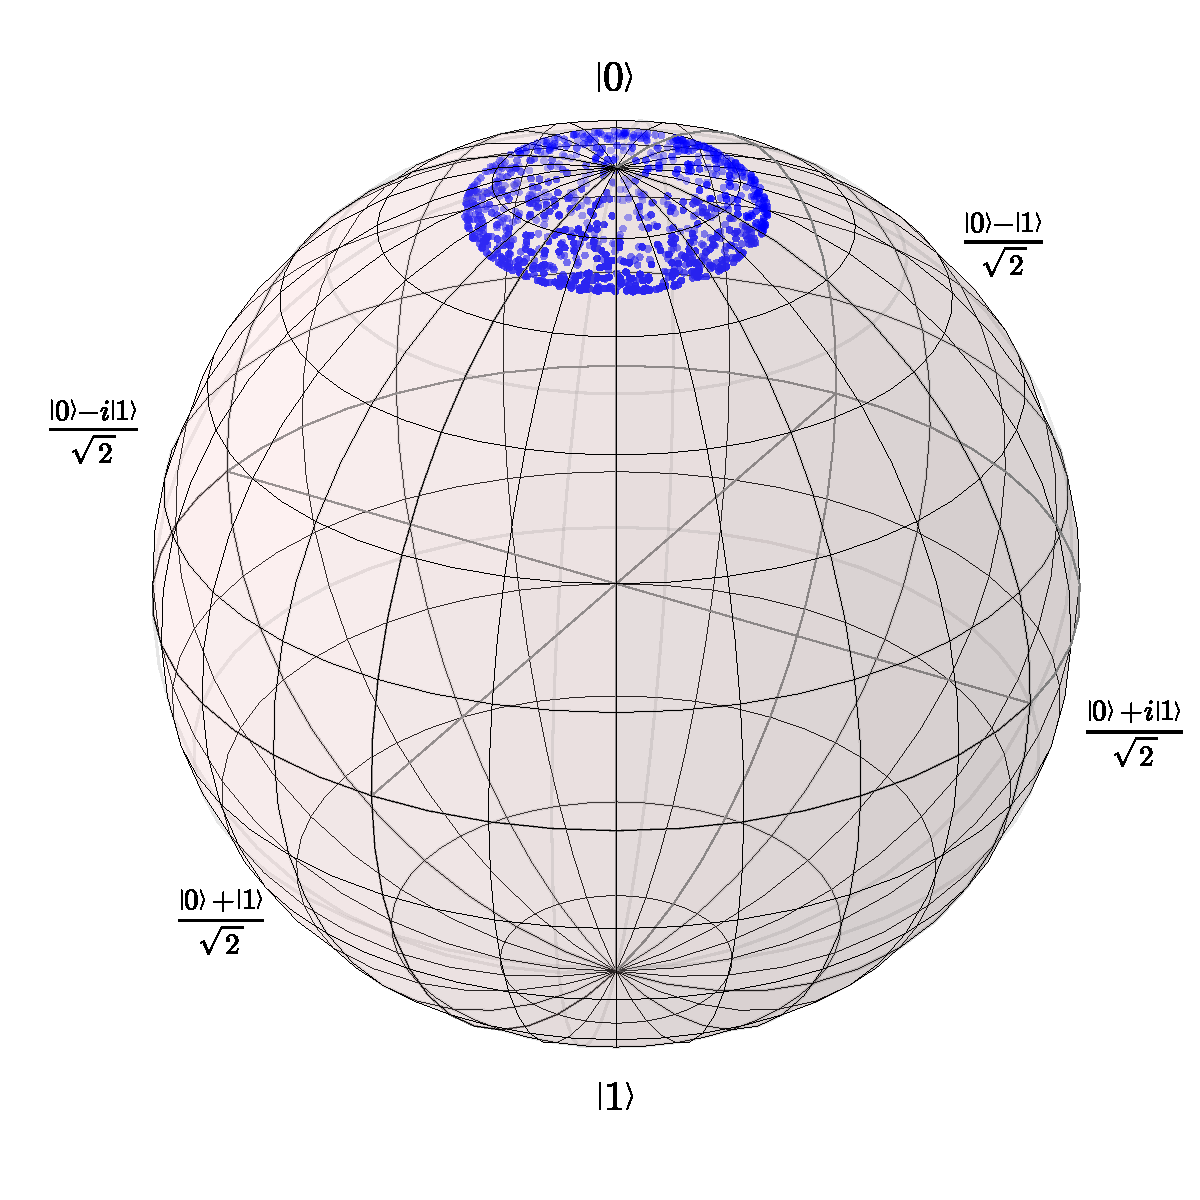
\includegraphics[height=0.75\textheight]{pics/channels/amplitude_dumping_0_9}
	\caption{
	Action of amplitude dumping channel:  
	\alert{$p=0.9$}.
	}
	\end{figure}
	}
	\end{frame}
%%%%%%%%%%%%%%%%%%%%%%%%%%%%%%%%%%%%%%%%%%%%%%%%%%%%%%%%%%%%%%%%%%%%%%%%%%%%%%%%
\subsection{Error correction}
	\begin{frame}{Shor error correction scheme}
	\begin{center}
	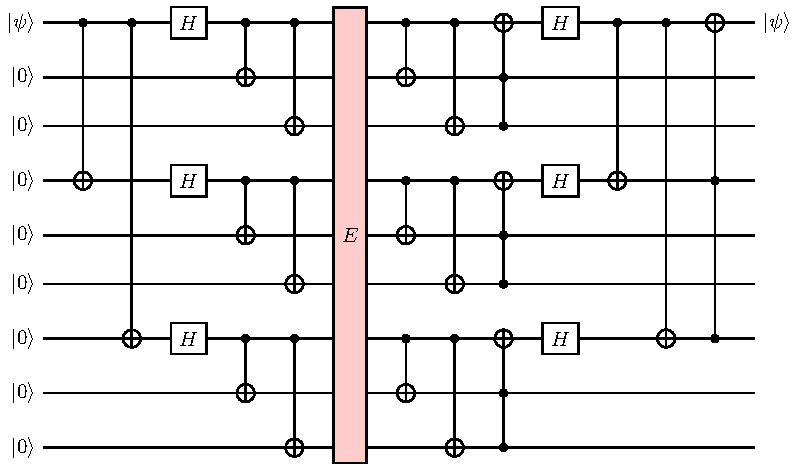
\includegraphics[height=0.6\textheight]{pics/shorcode.pdf}\\
	\end{center}
\end{frame}